\subsubsection{Termination}

When describing the shutdown of the whole system, we assumed the application
terminates gracefully.
In this section we show the algorithm we designed to achieve this goal.

As we can see from figure \ref{fig:termination-app}, the termination follows the
opposite order of the bootstrap.

\begin{figure}[H]
  \centering
  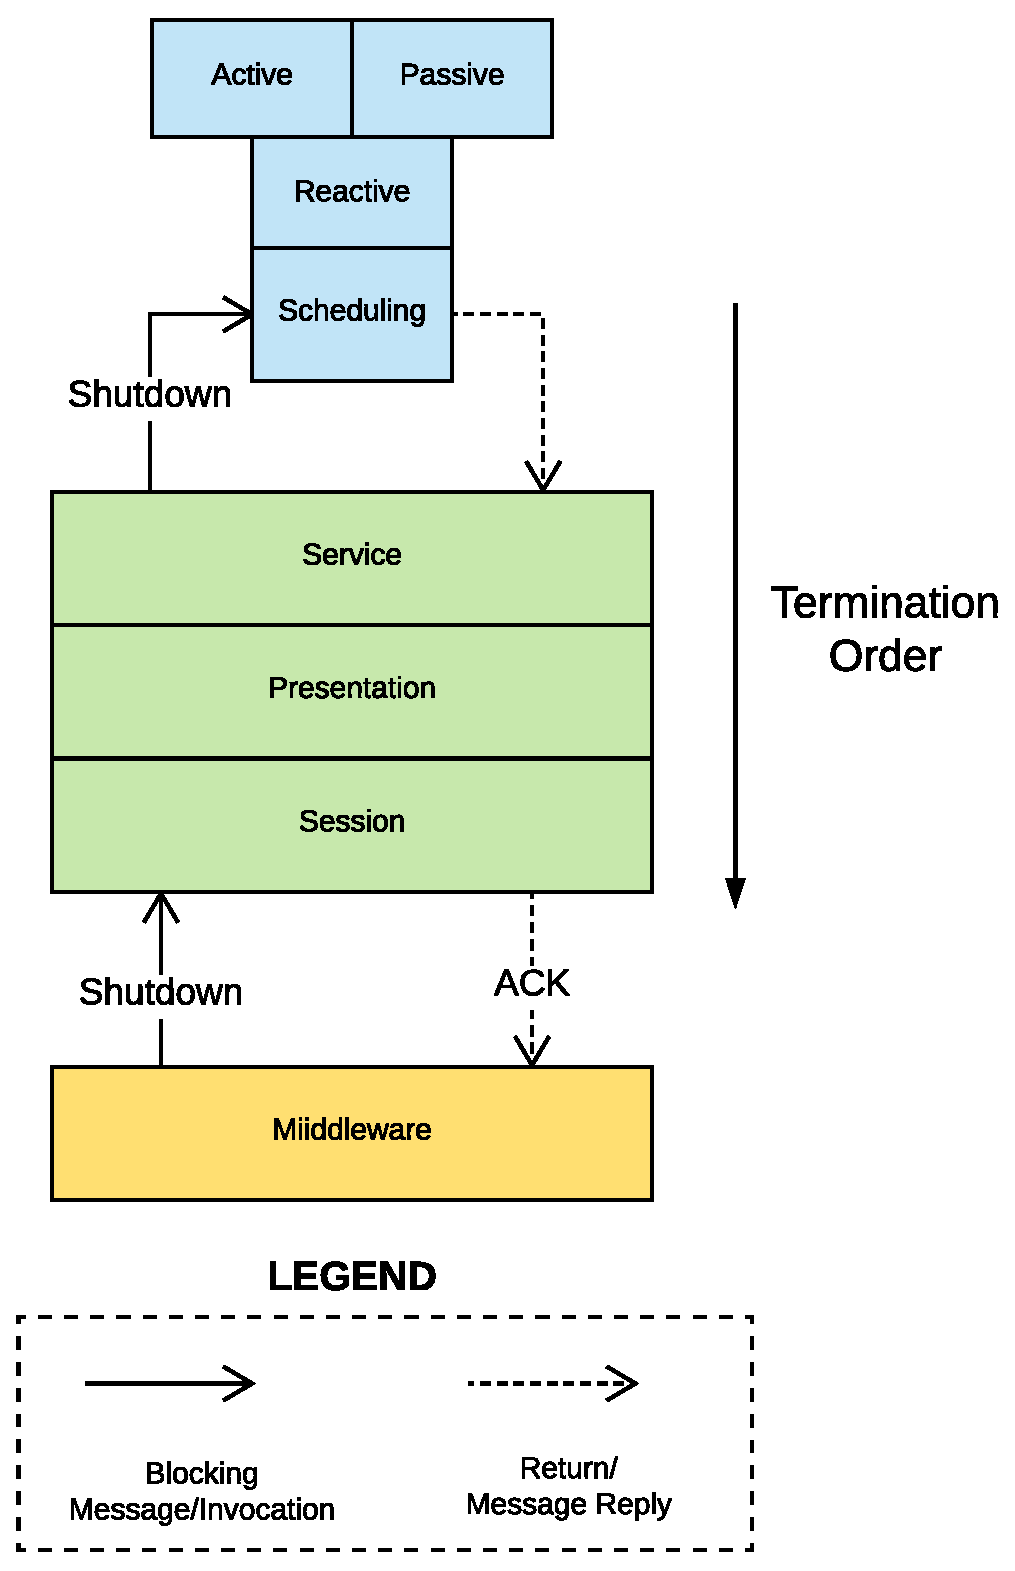
\includegraphics[scale=0.4,keepaspectratio]
    {images/solution/termination-app.eps}
  \caption{Application Termination}
  \label{fig:termination-app}
\end{figure}

%TODO: Review termination process
\begin{enumerate}
  \item The middleware send a \verb|shutdown| message;
  \item After stopping active entities, $I$ saves their state into a file;
  \item $I$ saves into a file the state of reactive entities.
    It is important to notice their internal state is now safely savable,
    since no active entities can modify it anymore;
  \item $I$ sends a \texttt{shutdown} message to the middleware through
  interface\_layer;
  \item $I$ terminates itself and the entire application consequently stops.
\end{enumerate}

The middleware layer can request the application to stop via the
\texttt{shutdown} message.

The last operation the \textit{Init} task does is to send a message for
apprising the middleware layer of the successful termination of the
application one.
Similarly to the bootstrap phase, the middleware expects to receive this
message within a certain amount of time.
In order to do so, when sending the message, $I$ also starts a timeout.
Wherefore if it expires before receiving a response message from the
middleware layer, it calls again the \texttt{app.shutdown} procedure the
application exposes.
